\documentclass[aa]{lib/aa}
\bibpunct{(}{)}{;}{a}{}{,} % to follow the A&A style
\usepackage{graphicx}
\usepackage{comment}
\usepackage{txfonts}
\usepackage{stfloats}
\newcommand{\spz}[1] {{\texttt{\textbf{SPZ: #1}}} }
\newcommand{\eh}[1] {{\texttt{\textbf{ EH: #1}}} }
\newcommand{\LSun}{\mbox{${L}_\odot$}}
\newcommand{\MSun}{\mbox{${M}_\odot$}}
\newcommand{\Msun}{\mbox{${M}_\odot$}}
\newcommand{\RSun}{\mbox{${R}_\odot$}}
\newcommand{\MJup}{\mbox{${M}_{\rm Jup}$}}

\def\apgt{\ {\raise-.5ex\hbox{$\buildrel>\over\sim$}}\ }
\def\aplt{\ {\raise-.5ex\hbox{$\buildrel<\over\sim$}}\ }
\def\lteq{\ {\raise-.5ex\hbox{$\buildrel<\over-$}}\ }

\newcommand{\jumbo}{\mbox{JuMBO}}
\newcommand{\jumbos}{\mbox{JuMBOs}}

\def\ind#1#2{\hbox{\hskip 0.0truein\hbox to 0.2truein{#1\hfil}
	        \hbox{\hsize 6.0truein\vtop{\ni#2}\hfil}}\vskip 1pt}

%-----------------------------------------------------------------------

\begin{document} 

   \title{The primoridal origin of Jupiter mass Binary Objects}
%   \author{E. Hochart\inst{1}
%          \and
%          S. Portegies Zwart\inst{1}
%          }
   \institute{
             Leiden Observatory, University of Leiden, 
             Niels Bohrweg 2, 2333 CA Leiden\\
             \email{hochart@mail.strw.leidenuniv.nl}
             \email{spzstrw.leidenuniv.nl}
             }
   \date{Received XXXXX; accepted XXXXXX}

%--------------------------------------------------------------------
  \abstract
  % context heading (optional)
   {}
  % aims heading
   {}
  % methods heading
   {}
  % results heading
   {}
  % conclusions heading (optional)
   {}
   \keywords{gravitational waves -- stars: black holes -- galaxies: nuclei -- stars: kinematics and dynamics -- black hole physics
            }

   \maketitle
   
%-------------------------------------------------------------------
\section{Introduction}

Recently \cite{2023arXiv231001231P} reported on the discovery of 42
jupiter-mass binaries in the direction of the Trapezium cluster.
Their component masses are between 0.6\,\MJup\, and 14\,\MJup\, with
projected separations between 25\,au and 380\,au.  Two
of these objects have a nearby tertiary jupiter-mass companion, and
they found an additional population of 540 single objects in the same
mass range. This discovery initiates the discussions on their origin
and surviveability in a clustered environment.

Jupiter-mass free floaters have been found before, but they are
generally isolated or with small (few au) separations
\citep{2021ApJS..253....7K}.  Known interstellar jupiter-mass binary
objects include\\
%%%
\begin{itemize}
\item[$\bullet$]2MASS J11193254-1137466 AB: a $5$ to 10\,\MJup\,
  primary in a $a=3.6\pm0.9$\,au orbit \citep{2017ApJ...843L...4B}.
\item[$\bullet$]WISE 1828+2650: a 3 to 6\MJup\, primary with a
  5\,\MJup\ companion in an $\apgt 0.5$\,au orbit
  \citep{2013ApJ...764..101B}.
\item[$\bullet$] WISE J0336-014: a $8.5$ to
  $18$\,\MJup primary with a $5$ to $11.5$\,\MJup\, companion in a
  $0.9^{+0.05}_{-0.09}$\,au orbit \citep{2023ApJ...947L..30C}.
\item[$\bullet$]2MASS J0013-1143 discovered by \cite{2017AJ....154..112K} and
  suspected to be a binary by \cite{2019A&A...629A.145E}.
\end{itemize}

Star formation, from the collapse of a molecular cloud through
gravitational instability, generally is expected to lead to objects
considerably more massive than Jupiter
\citep{1976MNRAS.176..367L,2005A&A...430.1059B}.  As a consequence,
the large population of jupiter-mass free-floaters is considered to
result from the ejected planets from dynamically unstable planetary
systems.  Several studies considered the possibility of planetary
systems losing outer-planets in dynamical interactions in dense
stellar systems (see i.e.,
\citep{1996Sci...274..954R,2015MNRAS.453.2759Z, 2017MNRAS.470.4337C,
  2019MNRAS.489.2280F, 2019A&A...624A.120V}), but they focus on the
ejection of single planets, not binaries.  Their origin through
dynamical phenomena is further complicated by the tendency for lower
mass planets to be more prone to ejections
\citep{2001Icar..150..303F,2013MNRAS.433..867H,2019MNRAS.489.2280F,2020MNRAS.497.1807S}.

We naively recognize four main scenarios for producing \jumbos.
Alternative to forming in situ (which we call scenario ${\cal ISF}$),
one can naively imagine three mechanisms to form jupiter mass binary
objects (\jumbos) \citep{2023arXiv231006016W} argued that these
binaries could be explained from planetary systems of which the outer
two planets are stripped by a passing star in a close encounter. The
two ejected planets would lead to a population of free floating
planets, but could also explain the observed population of \jumbos.
We call this scenario ${\cal SPP}$.

Alternatively one could imagine \jumbos\, to result from planet-moon
pairs orbiting some star that is ejected to become a jumbo.  We call
this scenario ${\cal SPM}$).

Finally, one could imagine that with a sufficiently large population
of free-floating jupiter-mass objects could lead to a population of
jumbos by dynamical capture of one jupiter by another.  We call this
scenario ${\cal FFC}$. A similar scenario was proposed by
\cite{2010MNRAS.404.1835K} for explaining very wide stellar pairs, but
the model was also adopted to account for wide planetary orbits
\citep{2012ApJ...750...83P}.

We start by discussing some fundamental properties of the
environmental dynamics, followed by a description of numerical
simulations to characterize the parameters of the acquired jumbos and
the resulting occurrence rates.

%--------------------------------------------------------------------
\section{The dynamical characterization of \jumbos}

The \jumbos\, discovered by \cite{2023arXiv231001231P} were location
in the Trapezium cluster. Assessing the cluster dynamics we base our
analysis on the analysis carried out by \cite{2016MNRAS.457..313P}.
He determined cluster parameters by numerical modeling of the
distribution of disk sizes observed in the Trapezium cluster, and
concluded that this distribution is best reproduced for a cluster
containing some 2500 stars with a total mass of $\sim 880$\,\MSun\,
and a half-mass radius of $\sim 0.5$\,pc. The results were only
consistent with the observations if the initial cluster density
distribution represented a fractal dimension of 1.6, and was
inconsistent with a \cite{1911MNRAS..71..460P} distribution.  For
consistency with earlier studies, we perform our analysis for Plummer
as well as for a fractal (with fractal dimension 1.6) distributions.

Adopting a Plummer distribution of the Trapezium cluster (with a
$r_{\rm vir} = 0.5$\,pc virial radius) would have a core radius of
$r_c \simeq 0.64r_{\rm vir} \sim 0.32$\,pc with a core mass of
250\,\MSun, which results in a velocity dispersion of $v_{\rm disp}
\equiv GM/(r\sqrt{r_c^2 + r_{\rm vir}^2} \simeq 0.97$\,km/s. With a
mean stellar mass in the cluster core of 1\,\MSun\, the unit of energy
expressed in the kinematic temperature kT becomes $\sim 8 \cdot
10^{42}$\,erg.

Jumbos are found in the mass range of about 0.6\,\MJup\, to
14\,\MJup\, and with a projected separation of 25\,au\, and $\sim
380$\,au.  The averaged observed values are $d=200\pm109$\,au,
$\langle M\rangle = 4.73\pm3.48$\,\MJup, and $\langle m\rangle =
2.81\pm2.29$\,\MJup.  For clarity we adopt here that the observed
range in projected distances between the two jupiter-mass objects is
consistent with an orbital separation, and express distances in terms
of semi-major axis instead.

To first order, the binding energy of jumbos then ranges between $\sim
5\cdot 10^{37}$\,erg and $1.4\cdot 10^{41}$\,erg, or at most $\sim
0.02$\,kT. Which makes them soft upon an encounter with a cluster
star.

The hardest \jumbo, composed of two 14\,\MJup\, planets in a 25\,au
orbit would be hard for another encountering object of less then
$17\,M_{\rm Jupiter}$.  For an encountering 1\,\MJup\, object a 25\,au
orbit would be hard only if the two planets are about three times as
massive a Jupiter.  The majority of jumbos in the trapezium cluster
are then still soft for any encountering free floating planet, but
hard if their orbits are tighter, or the encountering free floating
planet has low mass.

On average, soft encounters tend to soften these binaries even further
\citep{1975MNRAS.173..729H}, although an occasional soft encounter
with another planet may actually slightly harden the jumbo.  An low
impact-parameter encounter with a star will tend to ionize any of the
observed jumbos.  Independent of how tight the orbit.  Jumbos,
therefore, are expected to be relatively short lived, and dissociate
upon a close encounter with any other cluster member.

To further understand the dynamics of the jumbos in a clustered
environment, and to study the efficiency of the various formation
scenario's we perform $N$-body calculations of a Trapezium-like star
cluster with a population of jupiter-mass objects in various initial
configurations.

%--------------------------------------------------------------------
\section{Model calculations}

For each of our proposed models, ${\cal ISF}$ (in situ formation of
jumbos), ${\cal SPP}$ (as outer planets orbiting a star), ${\cal SPM}$
(as bound planet-moon pairs orbiting a star), and ${\cal FFC}$ (as
mutual capture of free-floaters) we perform a series of $N$-body
simulations with properties consistent with the Trapezium cluster.

Each cluster starts with 2500 single stars taken from a broken
power-law mass-function \citep{2002Sci...295...82K} between
0.08\,\MSun\, and $30$\,\MSun\, distributed either in a Plummer sphere
(model Pl) or a fractal distribution with a fractal dimension of 1.6
(model Fr). All models start in virial equilibrium.  We run three
models for each set of initial conditions, with a virial radius of
0.25\,pc, 0.5\,pc and 1.0\,pc, called model R025, R05 and R100,
respectively.  We ignore stellar evolution, as well as the tidal field
of the Galaxy.

For each of our proposed models, we initialize a population of single
or binary jupiter-mass objects. The single (and primaries in
primordial jumbos) are selected from a power-law mass function between
0.8\,\MJup\, and 14\,\MJup, which is consisted with the observed mass
function \citep{2023arXiv231001231P}. We fitted a power-law to the
primary-planet mass function, which has a slope of $\alpha_{\jumbo}
=-1.2$ (considearbly flatter than Salpter's $\alpha_{\rm Salpter} =
-2.35$).

For the models with free-floating jupiter-mass objects, scenario
${\cal FFC}$, we sprinkle the single planets in the cluster potential
as single objects using the same initial distribution function as we
used for the single stars.  These models were run with
1200\,jupiter-mass objects (or 600 pairs), but we performed additional
runs with $10^3$ and $10^4$ free floaters.

primordial \jumbos\, are initialized with semi-major axis with a flat
distribution between 10\,au and $10^3$\,au, an eccentricity from the
thermal distribution between 0 and 1, and a mass ratio (also from the
thermal distribution) between 0.2 and 1.  The binary is subsequently
rotated to a random orientation. We typically start with 1200 single
or 600 jupiter-mass pairs.

Isolated binaries, for scenario ${\cal ISF}$, are subsequently
sprinkled in the cluster potential as single objects using the same
initial distribution function as used for the single stars.

For scenario ${\cal SPM}$ we put the bound planet-moon pair in orbit
around a star.  The orbit of the planet-moon pair is circular and with
a random orientation at a distance from the star such that the
planet-moon's orbital separation is one-third of it's Hill radius.
This guarantees a stable planet-moon pair in orbit around the selected
star.

We selected the star to host such a planet-moon pair from 150 stars
lower in mass than 0.6\,\MSun\, and 150 more stars. The mid-mass point
(of 0.6\,\MSun) is almost twice the mean stellar mass in the mass
function.

For scenario ${\cal SPP}$, we select the same planet masses as for the
primordial \jumbos\, except that we have them orbiting one of the
selected stars as a hierarchical planetary system. The distance from
the first planet $a_1$ and the second planet $a_2$ (such that
$a_2>a_1$) are selected according to various criteria.  The inner
orbit $a_1$ was selected between 20\,au and $2000$\,au from a flat
distribution in $a$.  The outer orbit, $a_2$, we typically chose to be
ten times larger than the inner planet's Hill radius, but we also
perform simulations with five times and twice the Hill radius (we call
them model rH10, rH05 and rH02, respectively).

We perform an additional series of runs with pre-specified orbital
separations for the two planets $a_1$ and $a_2$, to follow the model
proposed in \cite{2023arXiv231006016W}.

Each run was repeated 10 times to deal with potential statistical
fluctuations, but we run 40 initiations of models ${\cal SPP}$\_Pl\_R025.

Each simulation is stopped at an age of 1\,Myr, after which we study
the population of free floating jupiter-mass objects and the
population of \jumbos.

To summarize, we performed the following model calculations:\\
\begin{tabular}{ll}
${\cal SPP}$ & As outer orbiting planets\\
${\cal SPM}$ & As bound planet-moon pair orbiting a star\\
${\cal FFC}$ & Free floating single planets.\\
${\cal ISF}$ & In situ formation of jumbos\\
\end{tabular}

\section{Results}

\subsection{Model ${\cal SPP}$}

In scenario ${\cal SPP}$, we follow the dynamical evolution of 1900
single stars, and 600 stars what are orbited by two planets.  According
to \cite{2023arXiv231006016W}, jumbos form naturally upon a dynamical
encounter between the planetary systems and a passing star.  In
table\,\ref{Tab:model_PP} we summarize the results of model ${\cal
  PP}$.

\begin{table}
 \caption{...}
 \label{Tab:model_PP}
 \centering 
 \begin{tabular}{lrrrrrrr}
 \hline\hline
model &$R_{\rm vir}$ & $n_J$ & $f_{j/s}$ & $\langle M \rangle$ & $\langle m \rangle$ & $\langle a \rangle$ & $\langle e \rangle$ \\
        \hline \vspace{-0.75em}\\
${\cal SPP}$\_Pl\_R025 & 0.4 &0& 7.35    & 2.3  & 2388 & 0.70 \\
${\cal SPP}$\_Pl\_R050 & 0.7 &0& 6.76    & 2.44 & 2196 & 0.86 \\
${\cal SPP}$\_Pl\_R100 & 0.4 &0& 3.77    & 1.67 & 1507 & 0.28 \\
${\cal SPP}$\_Fr\_R025 & 0.0 &0&  ---    & ---  &  --- & ---  \\			
${\cal SPP}$\_Fr\_R050 & 0.1 &0& 3.8     & 1.9  & 118  & 0.99 \\
${\cal SPP}$\_Fr\_R100 & 0.2 &0& 8.3     & 5.8  & 147  & 0.94 \\ 
 \hline
 \end{tabular}
\end{table}

The ${\cal SPP}$ model calculations fail to reproduce the observed
population of \jumbos. With a total of 600 planetary systems with two
jupiter-mass inner orbits between $a_1=20$\,au and 2000\,au the number
of \jumbos\, is still too low by about a factor 100, and their orbital
separations are about an order of magnitude too large.  The fractal
initial conditions produce even less \jumbos\, although the few that
formed have considerably smaller orbital separations.  Changing the
initial distribution in semi-major axis of the inner orbit from a
uniform distribution to a logarithmic distribution reduces the
formation rate of \jumbos\, even further.

To further explore the failure of model ${\cal SPP}$, we perform an
additional series of simulations with pre-determined inner and outer
orbital separations $a_1$ and $a_2$ using the Plummer distribution
with virial radii of 0.25\,pc, 0.50\,pc and 1.0\,pc for the stars.
According to \cite{2023arXiv231006016W}, the eventual orbital
separation of the \jumbo\, would be consistent with the difference in
orbital separation between the two planets when orbiting the star. For
this reason we perform an additional series of runs with a mutual
separation $a_2-a_1 = 200$\,au, expecting those to lead to consistent
results in comparison with the observations.  The results of these
simulations are presented in figure\,\ref{Fig:fjumbos_from_PP}.

For these models the \jumbo\, formation efficiency peaks for an
orbital separation $a_1 \apgt 800$\,au, but steeply drops for smaler
values of $a_1$. As proposd by \cite{2023arXiv231006016W}, we adopt an
difference in the initial orbital distance of about $a_2-a_1 =
100$\,au or 200\,au (see figure\,\ref{Fig:fjumbos_from_PP}), which
would lead to \jumbo\, orbits in the same range.  We performed a total
of 45 calculations with various ranges of $a_1$ and $a_2$, of which 39
produced a total of 910 \jumbos. The initial mean value of $a_1-a_2 =
167\pm38$\,au, leading to a final orbital separation of the jumbos of
$a_j \sim 262\pm45$\,au.  The claim made by
\cite{2023arXiv231006016W}, that the separation distance $a_2-a_1$
leads to \jumbos\, with a similar orbital distance seems reasonable.

\begin{figure}
    \centering
        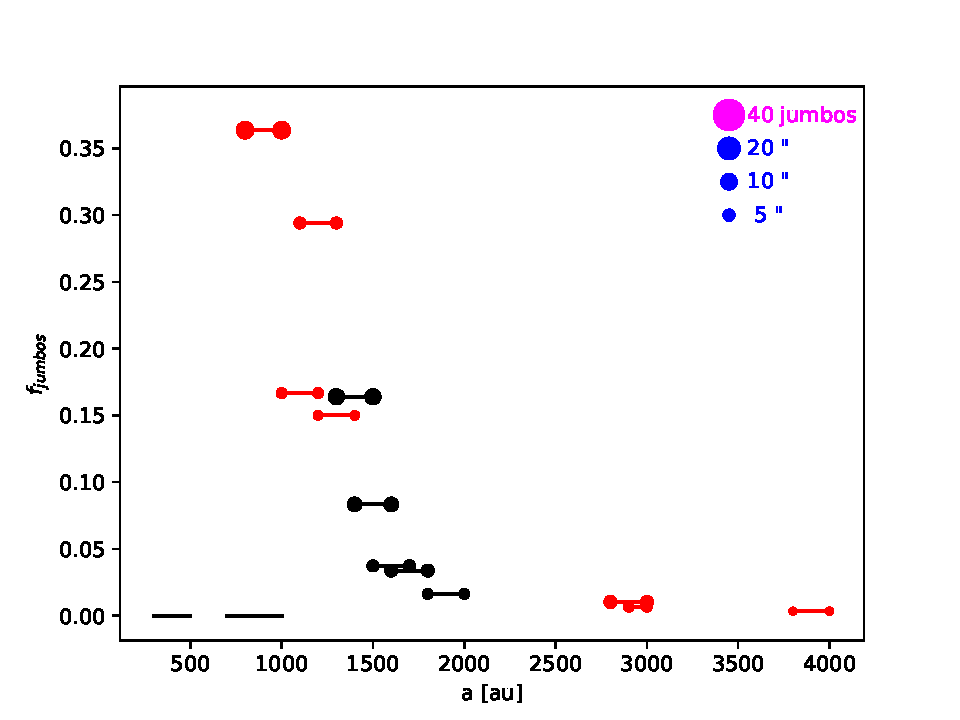
\includegraphics[width=.91\columnwidth]{figures/fig_fjumbos_from_psystems.pdf}
        \caption{The number of jumbo's produced in model ${\cal SPP}$,
          as fraction of the number of free floating planets for
          various simulations starting with a Plummer sphere with a
          virial radius of 0.5\,pc.  The bullet points along each line
          correspond with the adopted orbital separation of the two
          planets ($a_1$ and $a_2$).  The red symbols indicate an
          average orbital separations for the jumbos between 25\,au
          and 380\,au.  The black symbols are outside this regime.
          The symbol sizes give the number of jumbos (see top right
          for scaling) in the particular simulation.  }
         \label{Fig:fjumbos_from_PP}
\end{figure}

\subsection{Model ${\cal SPM}$}


\begin{table}
 \caption{...}
 \label{Tab:model_SPM}
 \centering 
 \begin{tabular}{lrrrrrrr}
   \hline\hline
model &$R_{\rm vir}$ & $n_J$ & $f_{j/s}$ & $\langle M \rangle$ & $\langle m \rangle$ & $\langle a \rangle$ & $\langle e \rangle$ \\
        \hline \vspace{-0.75em}\\
${\cal SPM}$\_Pl\_R05 & 286.5 &3.48& 4.19  & 3.24 & 224.9 & 0.21 \\
${\cal SPM}$\_Fr\_R05 &  61.7 &0.54& 4.90  & 3.55 & 175.8 & 0.47 \\ 
 \hline
 \end{tabular}
\end{table}

\subsection{Model ${\cal FFC}$}

\subsection{Model ${\cal ISF}$}

\begin{figure}
    \centering
        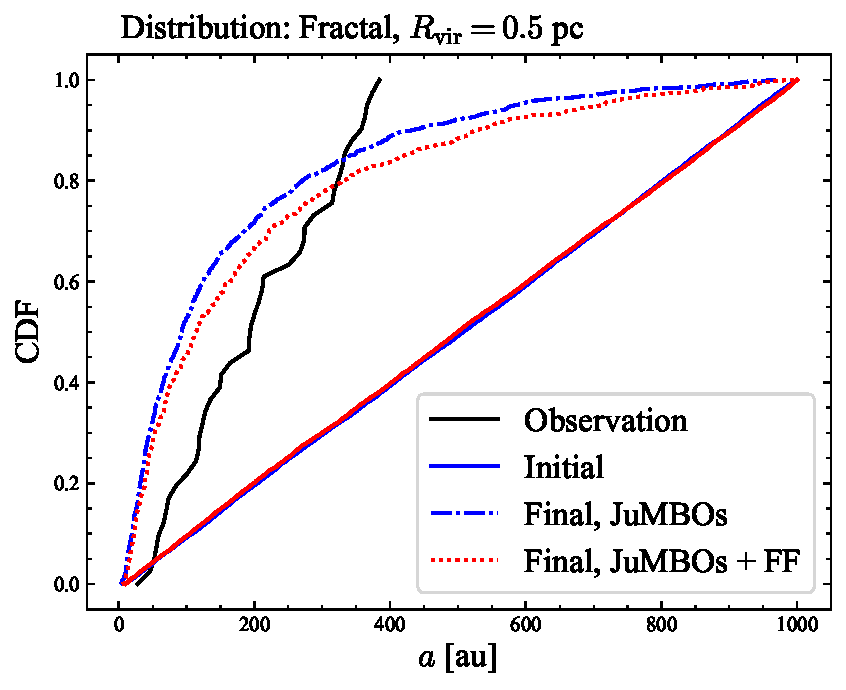
\includegraphics[width=.91\columnwidth]{figures/sem_axis_Fractal_FF.pdf}
        \caption{}
         \label{Fig:Fr_semimajor_axis}
\end{figure}

\begin{figure}
    \centering
        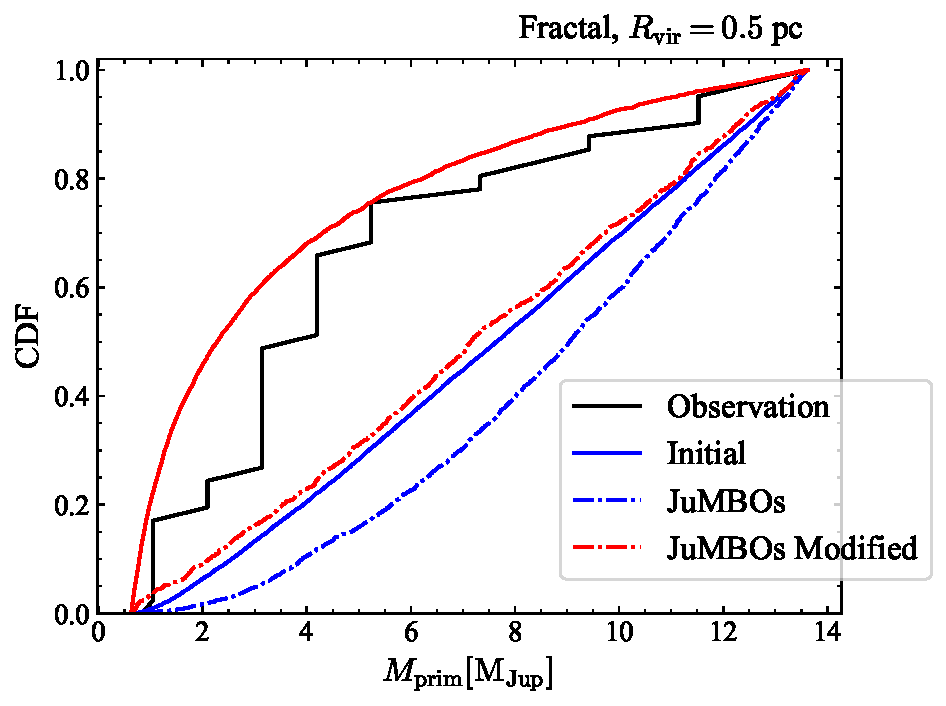
\includegraphics[width=.91\columnwidth]{figures/mprim_vs_obs_Fractal0.5Mod.pdf}
        \caption{}
         \label{Fig:Fr_primar_mass}
\end{figure}

\begin{figure}
    \centering
        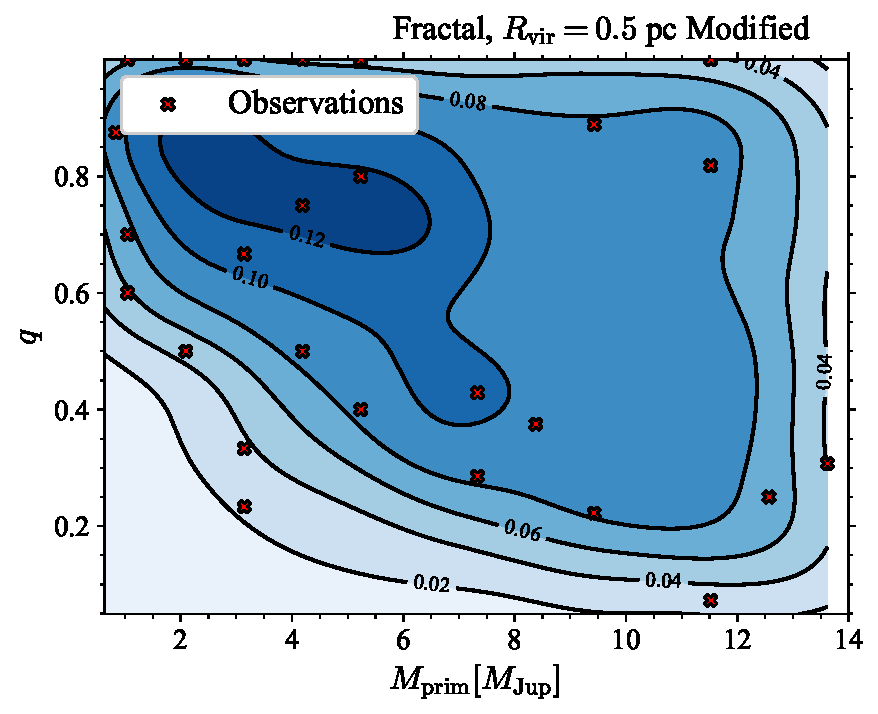
\includegraphics[width=.91\columnwidth]{figures/mass_distr_Fractal_rvir0.5_mod_params.pdf}
        \caption{}
         \label{Fig:Fr_mass_ratio_distribution}
\end{figure}

\begin{figure}
    \centering
        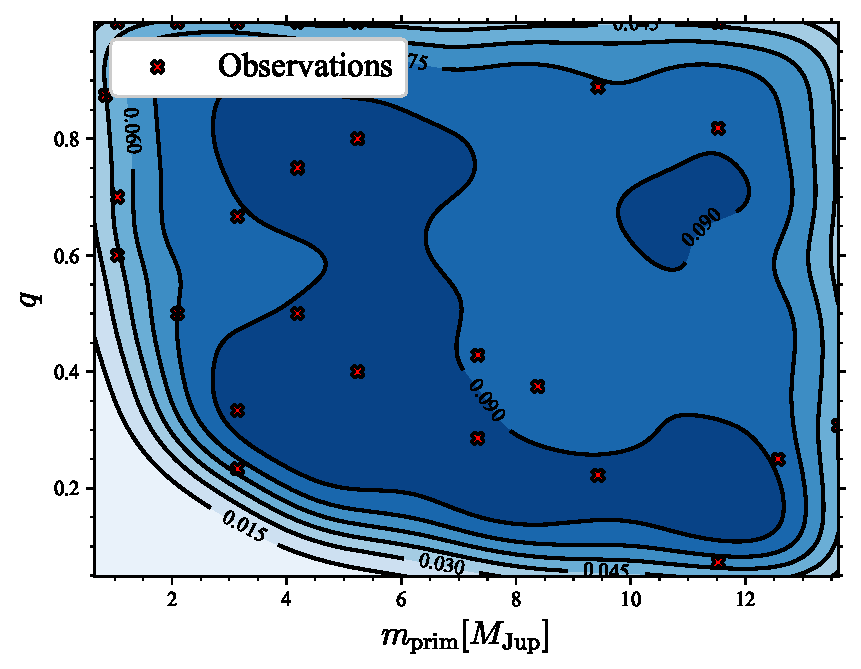
\includegraphics[width=.91\columnwidth]{figures/mass_distr_Plummer_rvir0.5.pdf}
        \caption{}
         \label{Fig:Plummer_massfunction}
\end{figure}
\begin{figure}
    \centering
        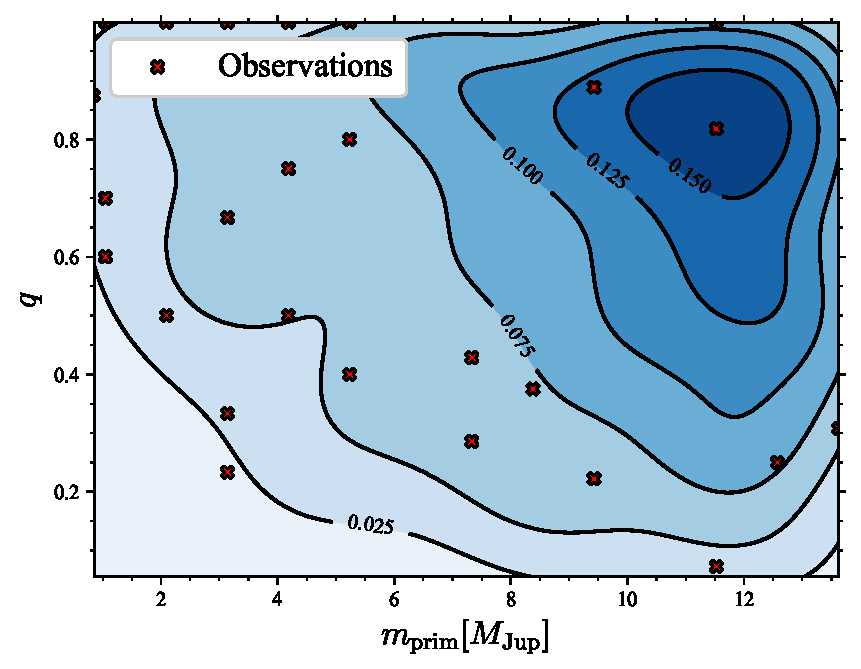
\includegraphics[width=.91\columnwidth]{figures/mass_distr_Fractal_rvir0.5.pdf}
        \caption{}
         \label{Fig:fractal_massfunction}
\end{figure}



\subsection{stellar and planetary collisions}

We did not find any collisions between stars or planets in a Plummer
models, but in the fractal models collisions are rather common.

in the ${\cal SPM}$ models $12.9\pm8.0$ stars experienced a collision
with another star. No planets collided with other planets, or with a
star.


\section{Discussion}


They calculate the rate by means of 4-body scattering experiments, in
which a star with two equal-mass planets with semi-major axes $a_1$
for the inner and $a_2$ for the other planet, encounters a single
star. Their largest cross section of roughly $a_1^2$ is obtained if
the encounter velocity $0.8v_\star/v_1$. For an encounter at the
cluster's velocity dispersion, the inner planet would then have a
orbital separation of about 900\,au around a 1\,\MSun\, star.

The orbital separation of the eventual jumbo would then be comparable
to the difference in orbital separation between the two planets
($a_{\rm Jumbo} \simeq a_2-a_1$).

The model in which \jumbos\, form a natural byproduct of the low-mass
end of the star-formation process

\subsection{The failure of model ${\cal SPP}$}

Note that an inner orbital separation of $a_1=800$\,au for a
10\,\MJup\, planet leads to a Hill radius of about 150\,au. An orbit
with $a_2=1000$\,au, the is probably only marginally stable.  Stille,
even in those runs the total number of \jumbos\, remains small
compared to the number of free floaters.

In \cite{2023arXiv231006016W}, the highest cross section is achieved
for the orbital velocity of the inner-most planet as fraction of the
typical encounter velocity $v1/v_{\rm disp} \sim 0.8$. With a cluster
velocity dispersion of $\sim 0.8$\,km/s, the orbital velocity roughly
1\,km/s. Around an 1\,\MSun\, star such a velocity is obtained,
assuming a Kepler orbit, at an orbital separation of 800\,au. It turns
out, that the results of the cross section calculations performed by
\cite{2023arXiv231006016W} are consistent with our direct N-body
simulation, but that the adopted initial orbital separation is too
wide in comparison with a realistically population of inner planetary
orbits for jupiter-mass planets.  Observational selection effect in
finding $\apgt 800$\,au jupiter-mass planets are quite severe, but we
consider it unrealistic to have 600 out of 2500 stars to be orbited by
such wide planetary systems. In particular, when one considers the
small sizes of the observed disks in the Trapezium cluster, which
today are all smaller than 400\,au \citep{2005A&A...441..195V}.



\subsection{\jumbos\, as former planet-moon pairs}

According to \cite{2023arXiv231015603C}, jumbos form naturally upon a
dynamical encounter between two stars one of which with orbited by a
binary planet or planet-moon system.

Both calculations \cite{2023arXiv231006016W} and
\cite{2023arXiv231015603C} adopt scattering experiments to determine
the formation rate of jumbos from their adopted initial conditions.


%--------------------------------------------------------------------
\section{Discussion}

\cite{2023arXiv231015603C} argued that \jumbos potentially originate
from tilted circum-binary planets. Formed as a --sort-of-- planet-moon
system in a wide orbit around a star, that is strippied from the host
star by the cluster potential or a relatively wide encounter with
another star. 



%--------------------------------------------------------------------
\section{Conclusion}

\section*{Acknowledgements}

Veronica Saz Ulibarrena, Shuo Huang, Maite Wilhelm, Brent Maas
    
\input /home/spz/Latex/lib/bib/references
    
\end{document}

%%%%%%%%%%%%%%%%%%%%%%%%%%%%%%%%%%%%%%%%%%%%%%%%%%%%%%%%%%%%%%
%-------------------------------------------------------------------
% END OF TEXT
%-------------------------------------------------------------------
%%%%%%%%%%%%%%%%%%%%%%%%%%%%%%%%%%%%%%%%%%%%%%%%%%%%%%%%%%%%%%

Pl
Rvir N/run <M>	<m>	<a>	<e>	Nruns
0.25 0.4   7.35	2.35	2388	0.70	40
0.50 0.7   6.76	2.44	2196	0.86	10
1.00 0.4   3.77	1.67	1507	0.28	10

Fr1.6 
Rvir N/run <M>	<m>	<a>	<e>	Nruns
0.25 0.0				10
0.50 0.1   3.8	1.9	118	0.99	10
1.00 0.2   8.3	5.8	147	0.94	10

Pl with Rvir= 0.25pc with various secondary planet orbits (rHill)
rH N/run <M>	<m>	<a>	<e>	Nruns
10 0.4   7.35	2.35	2388	0.70	40
5  2.6	 8.32	2.27	1895	0.78	10
2  8.6	 6.60	2.89	1448	0.82	10

Pl with Rvir= 0.25pc at various times (t)
t   N/run  <M>	<m>	<a>	<e>	Nruns
1.0 0.40   7.35	2.35	2388	0.70	40
0.5 0.15   5.43	1.58	4400	0.67	40

Pl with Rvir= 0.25pc rH=5, q=sqrt() 
t   N/run  <M>	<m>	<a>	<e>	Nruns
1.0 0.8	   2.50 1.36   2716.31   0.777  10

SPM models:
   F,amin,amax,Nss,Nsp,Nj,M,dM,m,dm,q,dq,a,da,e,de
PlN2500n600pm_R0.5pcQ05_R.0010.csv,0,1,-7653,823,2865,3.241863236847126,3.146419649374478,4.1994324138885455,3.6477551651523243,2.292947966246368,2.9219855055516857,224.8664798090486,107.62369768018677,0.21362638856650273,0.24988436693392485
FrN2500n600pm_R0.5pcQ05_R.0011.csv,0,1,-1028,1136,617,3.5484148732876206,3.317421904592993,4.905084847828215,4.019173763984519,2.5668243481935926,3.2345942681146256,175.82553098470015,150.19026253990216,0.4658461018866108,0.2849317239089184

